\chapter{Appendix}
\clearpage

\section{Declaration of Authorship} \label{Declaration of Authorship}
We hereby certify that the thesis we are submitting is entirely our own original work except where otherwise indicated. I am aware of the University’s regulations concerning plagiarism, including those regulations concerning disciplinary actions that may result from plagiarism. Any use of the works of any other author, in any form, is properly acknowledged at their point of use.

\bigskip
\textbf{Location, Date} \\
Rapperswil, 03. June 2022

\vspace{1.2cm}
\begin{tabular}{@{}p{0.1cm}p{6cm}p{0.6cm}p{6cm}@{}}
& \hrulefill \\[-0.3em]
& Luca Jost\\
\end{tabular}


\includegraphics[width=4.8cm, align=t, smash=br, hshift=0.9cm, vshift=2.55cm]{appendix/Signature_Luca_Jost.pdf}

\newpage

\section{Project Schedule} \label{fig:project_schedule}
\enlargethispage{2.5cm}
\begin{adjustwidth}{0.23cm}{0cm} \hfuzz=7.0pt \vfuzz=20.0pt
\makebox[\textwidth]{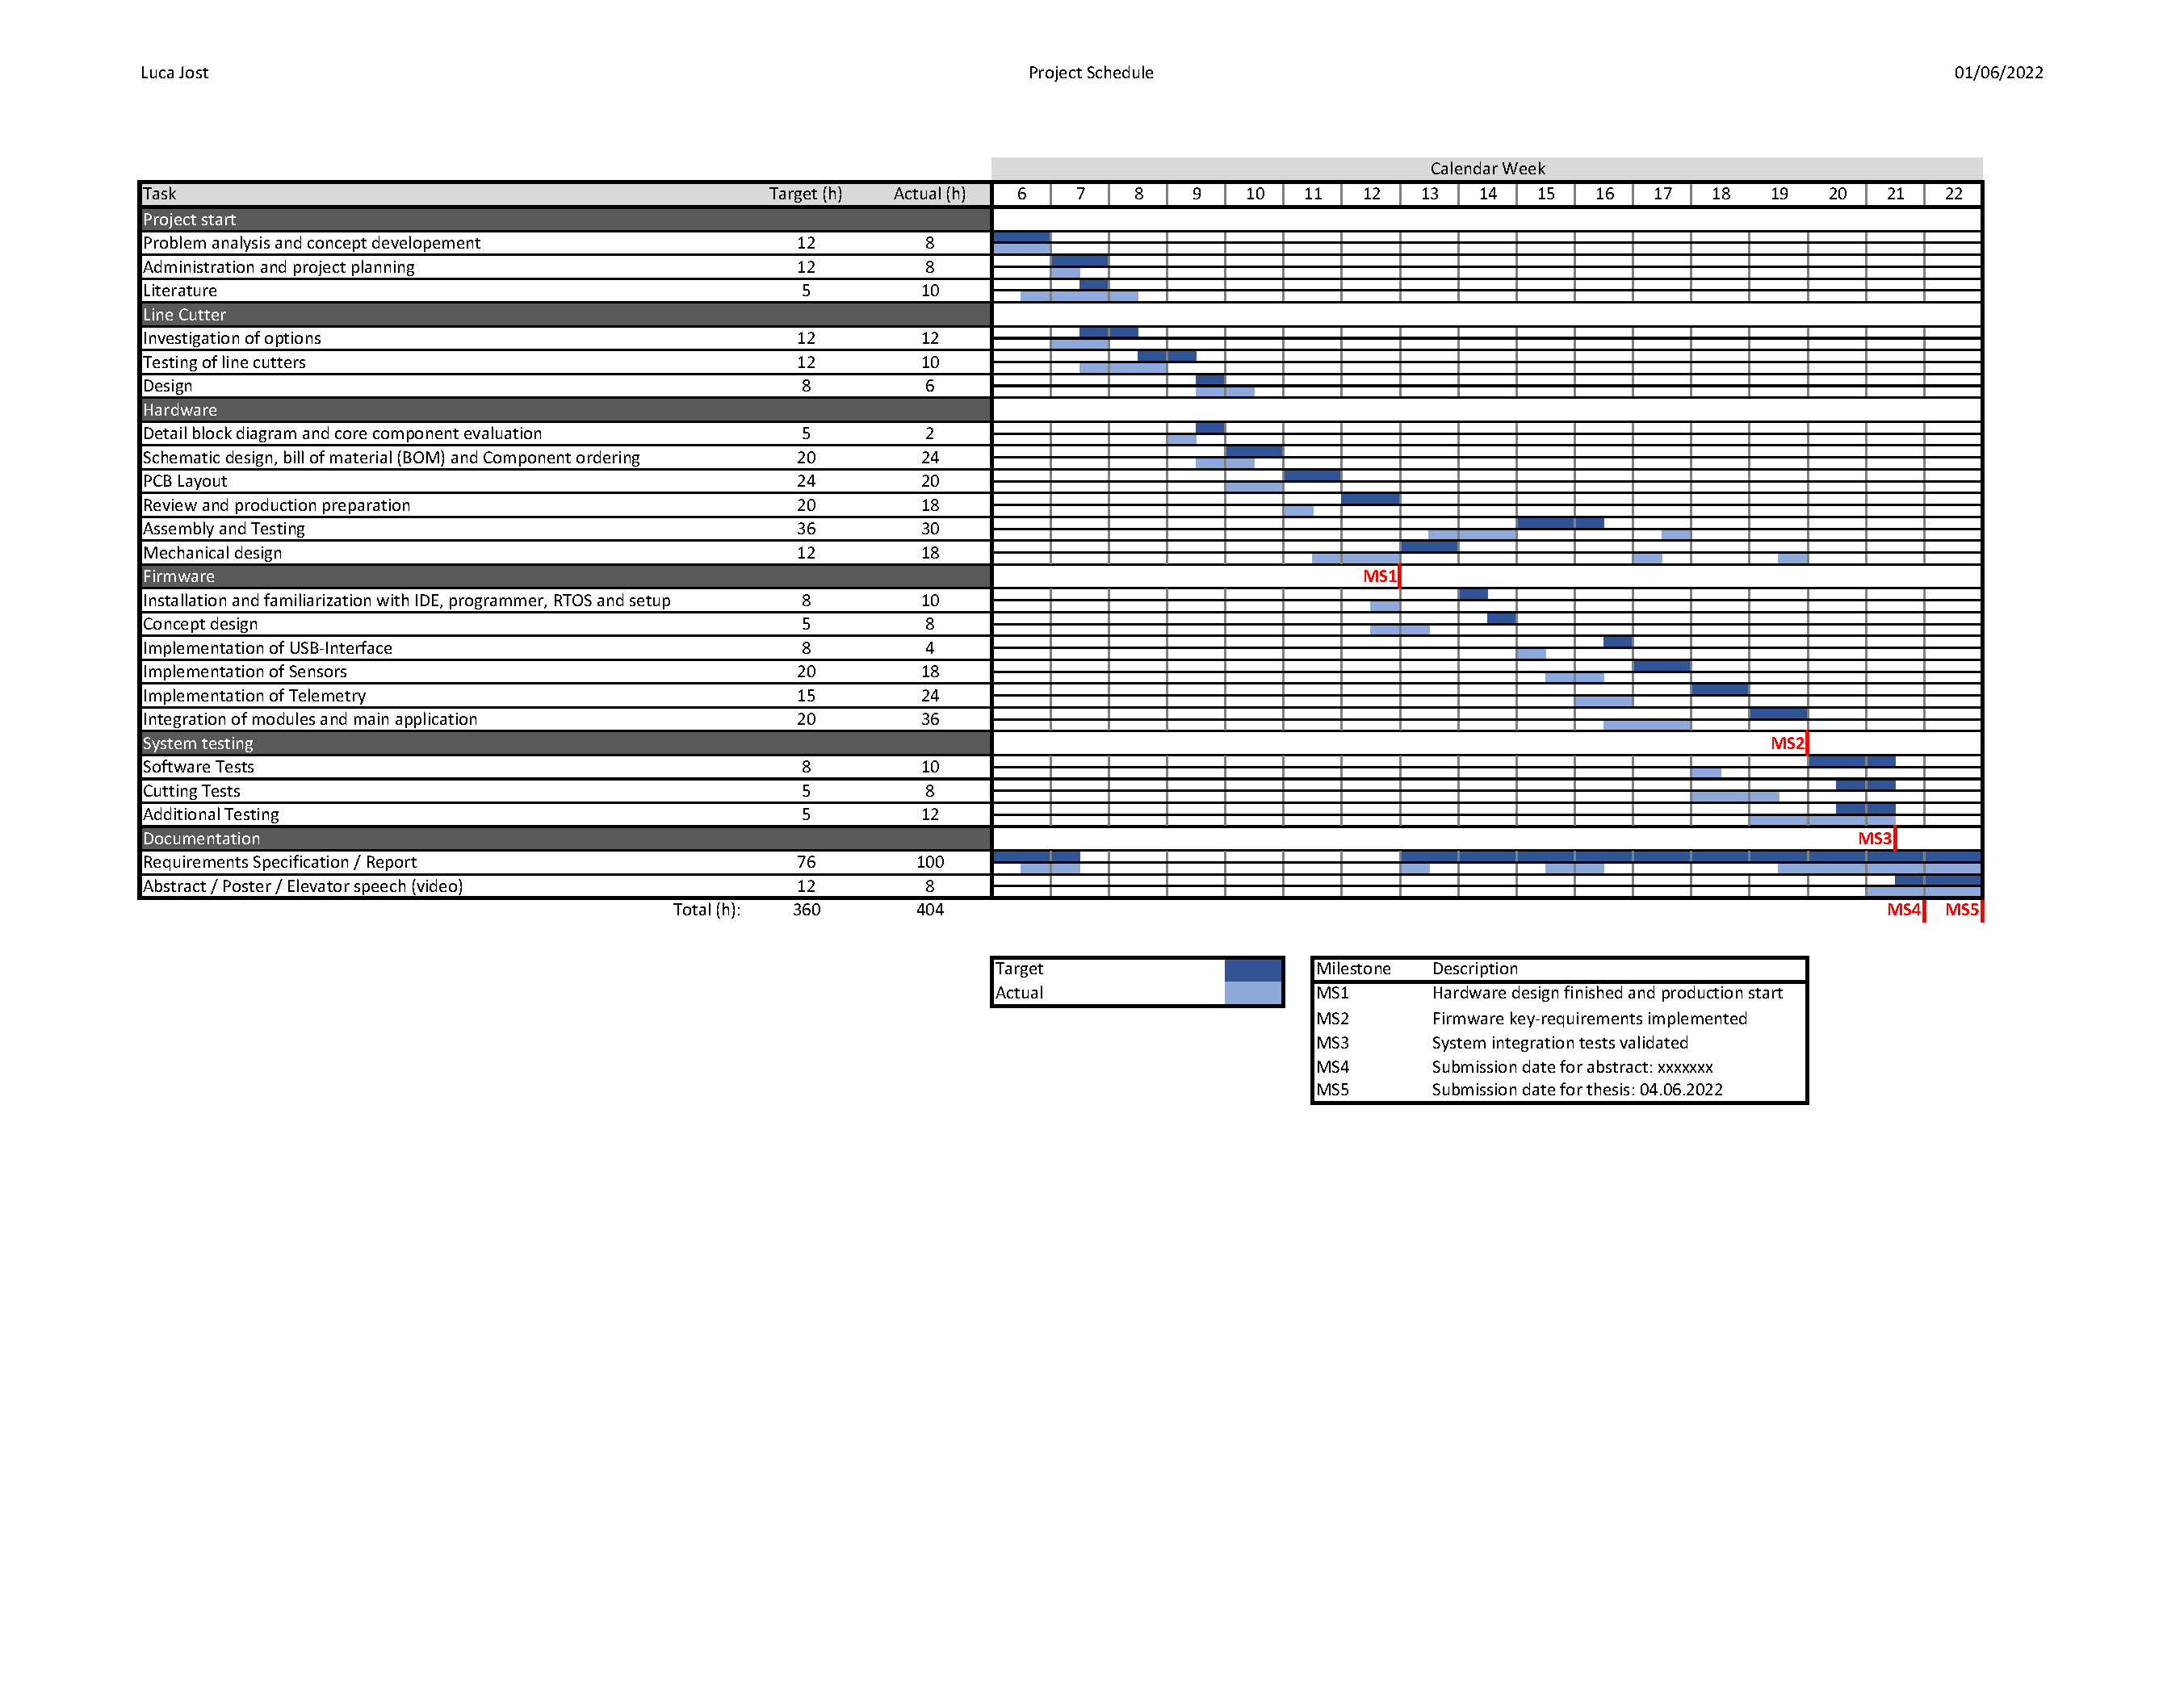
\includegraphics[angle=90, width=17.3cm, page=1]{appendix/Project_Schedule_220601.pdf}}
\end{adjustwidth}
\newpage

\section{Task Definition} \label{apx:assignment}
\enlargethispage{2.5cm}
\begin{adjustwidth}{-0.23cm}{0cm} \hfuzz=7.0pt \vfuzz=20.0pt
\makebox[\textwidth]{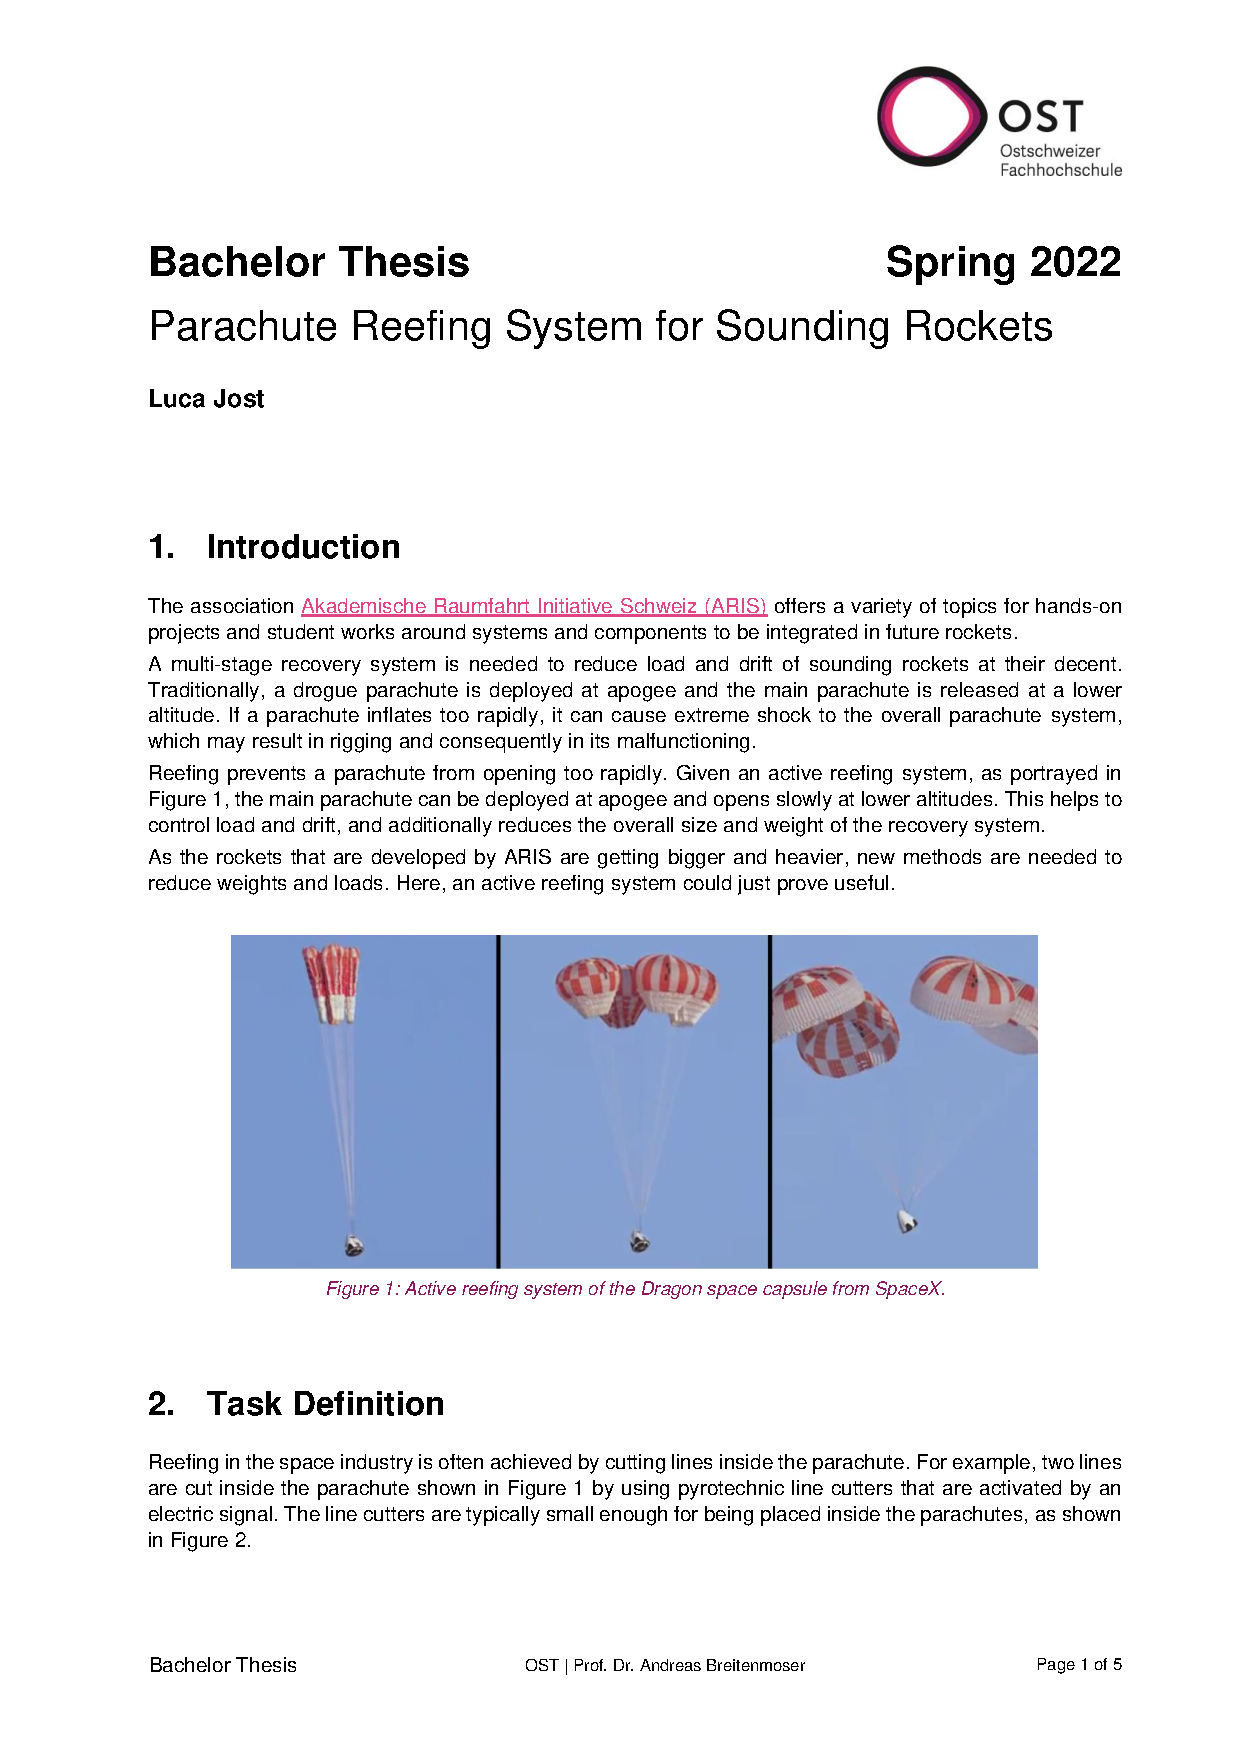
\includegraphics[width=17.3cm, page=1]{appendix/thesis-assigment}}
\end{adjustwidth}
\newpage

\begin{adjustwidth}{-0.23cm}{0cm} \hfuzz=7.0pt \vfuzz=20.0pt
\makebox[\textwidth]{\includegraphics[width=17.3cm, page=2]{appendix/thesis-assigment}}
\end{adjustwidth}
\newpage

\begin{adjustwidth}{-0.23cm}{0cm} \hfuzz=7.0pt \vfuzz=20.0pt
\makebox[\textwidth]{\includegraphics[width=17.3cm, page=3]{appendix/thesis-assigment}}
\end{adjustwidth}
\newpage

\begin{adjustwidth}{-0.23cm}{0cm} \hfuzz=7.0pt \vfuzz=20.0pt
\makebox[\textwidth]{\includegraphics[width=17.3cm, page=4]{appendix/thesis-assigment}}
\end{adjustwidth}
\newpage

\begin{adjustwidth}{-0.23cm}{0cm} \hfuzz=7.0pt \vfuzz=20.0pt
\makebox[\textwidth]{\includegraphics[width=17.3cm, page=5]{appendix/thesis-assigment}}
\end{adjustwidth}
\newpage


\section{Kalman Filter Discretization \& Implementation}\label{apx:kalman}
\subsection{Discretization}
In order to implement the system in the real world, the filter needs to be discretized. This step is done with the zero-order hold discretization to convert the continuous-time state space system to a discrete-time model with a fixed timestep.\cite{kalman-discretization}

Applying the zero-order hold method we get
\begin{equation}
\begin{split}
    Ad & = \mathrm{e}^{AT_s} \\
    Gd & = \int_0^{T_s} \mathrm{e}^{At} G \,\mathrm{d}t \\
    Hd & = H
\end{split}
\end{equation}

Applying the Taylor series for $Ad$ we get

\begin{equation}
\begin{split}
    Ad & = \displaystyle\sum_{n=1}^{\infty} \frac{{T_s}^n A^n}{n!} \\
    & = \mathbb{I} + AT + \frac{A^2 T^2}{2!} + ...\\
    & = \begin{bmatrix}1 & 0 \\ 0 & 1 \end{bmatrix} + \begin{bmatrix}0 & T_s \\ 0 & 0 \end{bmatrix} + \begin{bmatrix}0 & 0 \\ 0 & 0 \end{bmatrix} + ... \\
    & = \begin{bmatrix}1 & T_s \\ 0 & 1 \end{bmatrix}
\end{split}
\end{equation}

By using the result from above and solving the integral we can solve $Gd$
\begin{equation}
\begin{split}
    Gd & = \int_0^{T_s} \begin{bmatrix}1 & t\\ 0 & 1 \end{bmatrix} \begin{bmatrix}0 \\ 1 \end{bmatrix} \,\mathrm{d}t \\
    & = \int_0^{T_s} \begin{bmatrix} t \\ 1 \end{bmatrix} \,\mathrm{d}t \\
    & = \begin{bmatrix} \frac{t^2}{2} \\ t \end{bmatrix} \bigg|_0^{T_s} \\
    & = \begin{bmatrix} \frac{{T_s}^2}{2} \\ {T_s} \end{bmatrix}
\end{split}
\end{equation}

\newpage

\subsection{Implementation}
The system is now fully defined and the standard Kalman Filter equations can be used.\cite{kalman-introduction}

Prediction Step
\begin{equation}
    \hat{x_k} = A \bar{x}_{k-1}
\end{equation}
where
\begin{itemize}
    \item $\hat{x}$ is the predicted state estimate;
    \item $\bar{x}_{k-1}$ is the previous updated estimate.
\end{itemize}

\begin{equation}
    \bar{P_k} = A \hat{P}_{k-1} A^T + Gd Q Gd^T
\end{equation}
where
\begin{itemize}
    \item $\bar{P_k}$ is the predicted error covariance;
    \item $Q$ is the acceleration covariance $\sigma_a$.
\end{itemize}

Update Step
\begin{equation}
    K_k = \bar{P}_k H^T(R + H \bar{P}_k H^T)^{-1}
\end{equation}
where
\begin{itemize}
    \item $K_k$ is the Kalman gain;
    \item $R$ is the altitude measurement covariance $\sigma_R$.
\end{itemize}

\begin{equation}
    \bar{x_k} = \hat{x_k} + K_k(y-H\hat{x_k})
\end{equation}
where
\begin{itemize}
    \item $\bar{x_k}$ is the updated state estimate;
    \item $y$ is the altitude measurement. 
\end{itemize}

\begin{equation}
    \hat{P_k} = (\mathrm{I} - K_k H)\bar{P}
\end{equation}
\begin{itemize}
    \item $\hat{P_k}$ is the updated error covariance.
\end{itemize}

\newpage

\section{Reefing-System Schematics} \label{apx:schematic}
\enlargethispage{2.5cm}
\begin{adjustwidth}{-0.23cm}{0cm} \hfuzz=7.0pt \vfuzz=20.0pt
\makebox[\textwidth]{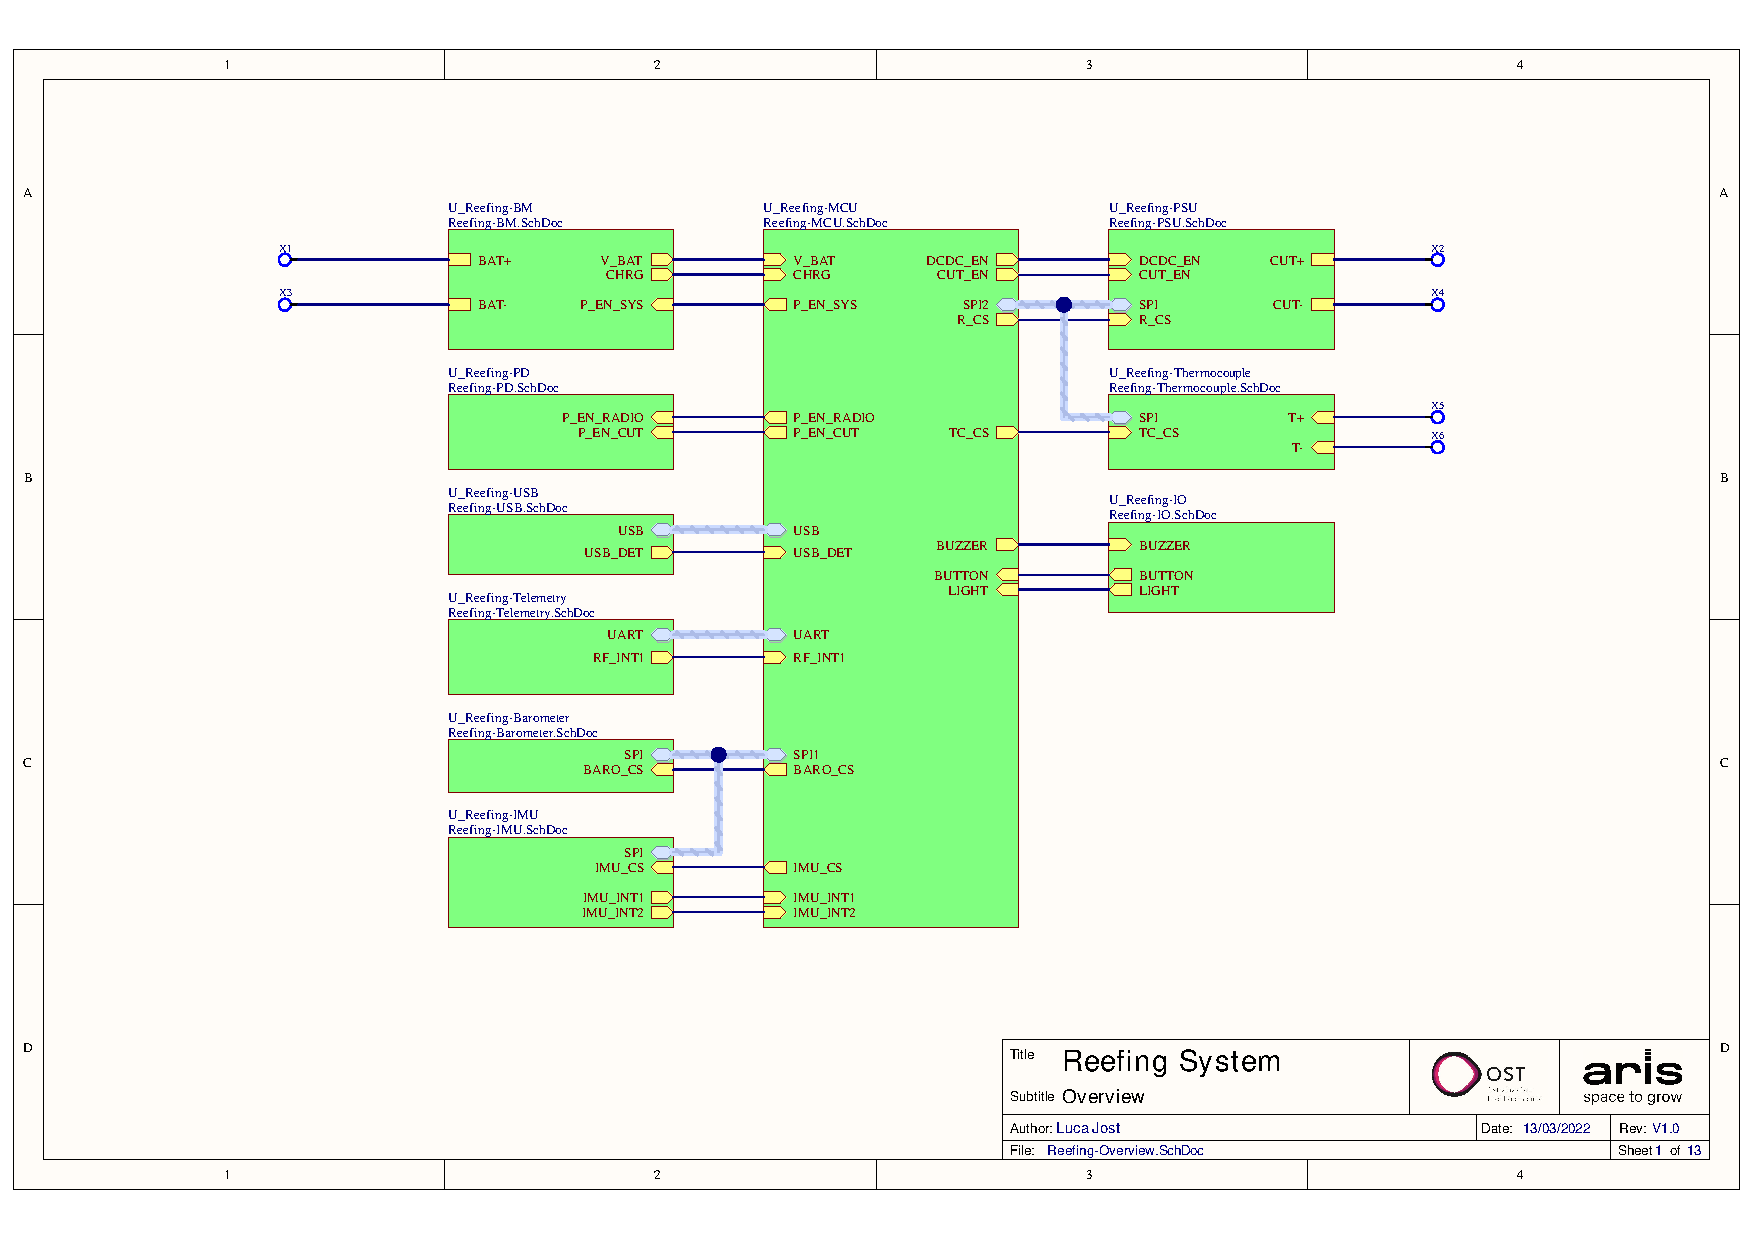
\includegraphics[angle=90, width=17.3cm, page=1]{appendix/Reefing System Schematics}}
\end{adjustwidth}
\newpage

\begin{adjustwidth}{0.23cm}{0cm} \hfuzz=7.0pt \vfuzz=20.0pt
\makebox[\textwidth]{\includegraphics[angle=90, width=17.3cm, page=2]{appendix/Reefing System Schematics}}
\end{adjustwidth}
\newpage

\begin{adjustwidth}{-0.23cm}{0cm} \hfuzz=7.0pt \vfuzz=20.0pt
\makebox[\textwidth]{\includegraphics[angle=90, width=17.3cm, page=3]{appendix/Reefing System Schematics}}
\end{adjustwidth}
\newpage

\begin{adjustwidth}{-0.23cm}{0cm} \hfuzz=7.0pt \vfuzz=20.0pt
\makebox[\textwidth]{\includegraphics[angle=90, width=17.3cm, page=4]{appendix/Reefing System Schematics}}
\end{adjustwidth}
\newpage

\begin{adjustwidth}{-0.23cm}{0cm} \hfuzz=7.0pt \vfuzz=20.0pt
\makebox[\textwidth]{\includegraphics[angle=90, width=17.3cm, page=5]{appendix/Reefing System Schematics}}
\end{adjustwidth}
\newpage

\begin{adjustwidth}{-0.23cm}{0cm} \hfuzz=7.0pt \vfuzz=20.0pt
\makebox[\textwidth]{\includegraphics[angle=90, width=17.3cm, page=6]{appendix/Reefing System Schematics}}
\end{adjustwidth}
\newpage

\begin{adjustwidth}{-0.23cm}{0cm} \hfuzz=7.0pt \vfuzz=20.0pt
\makebox[\textwidth]{\includegraphics[angle=90, width=17.3cm, page=7]{appendix/Reefing System Schematics}}
\end{adjustwidth}
\newpage

\begin{adjustwidth}{-0.23cm}{0cm} \hfuzz=7.0pt \vfuzz=20.0pt
\makebox[\textwidth]{\includegraphics[angle=90, width=17.3cm, page=8]{appendix/Reefing System Schematics}}
\end{adjustwidth}
\newpage

\begin{adjustwidth}{-0.23cm}{0cm} \hfuzz=7.0pt \vfuzz=20.0pt
\makebox[\textwidth]{\includegraphics[angle=90, width=17.3cm, page=9]{appendix/Reefing System Schematics}}
\end{adjustwidth}
\newpage

\begin{adjustwidth}{-0.23cm}{0cm} \hfuzz=7.0pt \vfuzz=20.0pt
\makebox[\textwidth]{\includegraphics[angle=90, width=17.3cm, page=10]{appendix/Reefing System Schematics}}
\end{adjustwidth}
\newpage

\begin{adjustwidth}{-0.23cm}{0cm} \hfuzz=7.0pt \vfuzz=20.0pt
\makebox[\textwidth]{\includegraphics[angle=90, width=17.3cm, page=11]{appendix/Reefing System Schematics}}
\end{adjustwidth}
\newpage

\begin{adjustwidth}{-0.23cm}{0cm} \hfuzz=7.0pt \vfuzz=20.0pt
\makebox[\textwidth]{\includegraphics[angle=90, width=17.3cm, page=12]{appendix/Reefing System Schematics}}
\end{adjustwidth}
\newpage

\begin{adjustwidth}{-0.23cm}{0cm} \hfuzz=7.0pt \vfuzz=20.0pt
\makebox[\textwidth]{\includegraphics[angle=90, width=17.3cm, page=13]{appendix/Reefing System Schematics}}
\end{adjustwidth}
\newpage

\section{Reefing-System Mechanical Drawing} \label{Reefing System Enclosure Mechanical Drawing}
\enlargethispage{2.5cm}
\begin{adjustwidth}{0.23cm}{0cm} \hfuzz=7.0pt \vfuzz=20.0pt
\makebox[\textwidth]{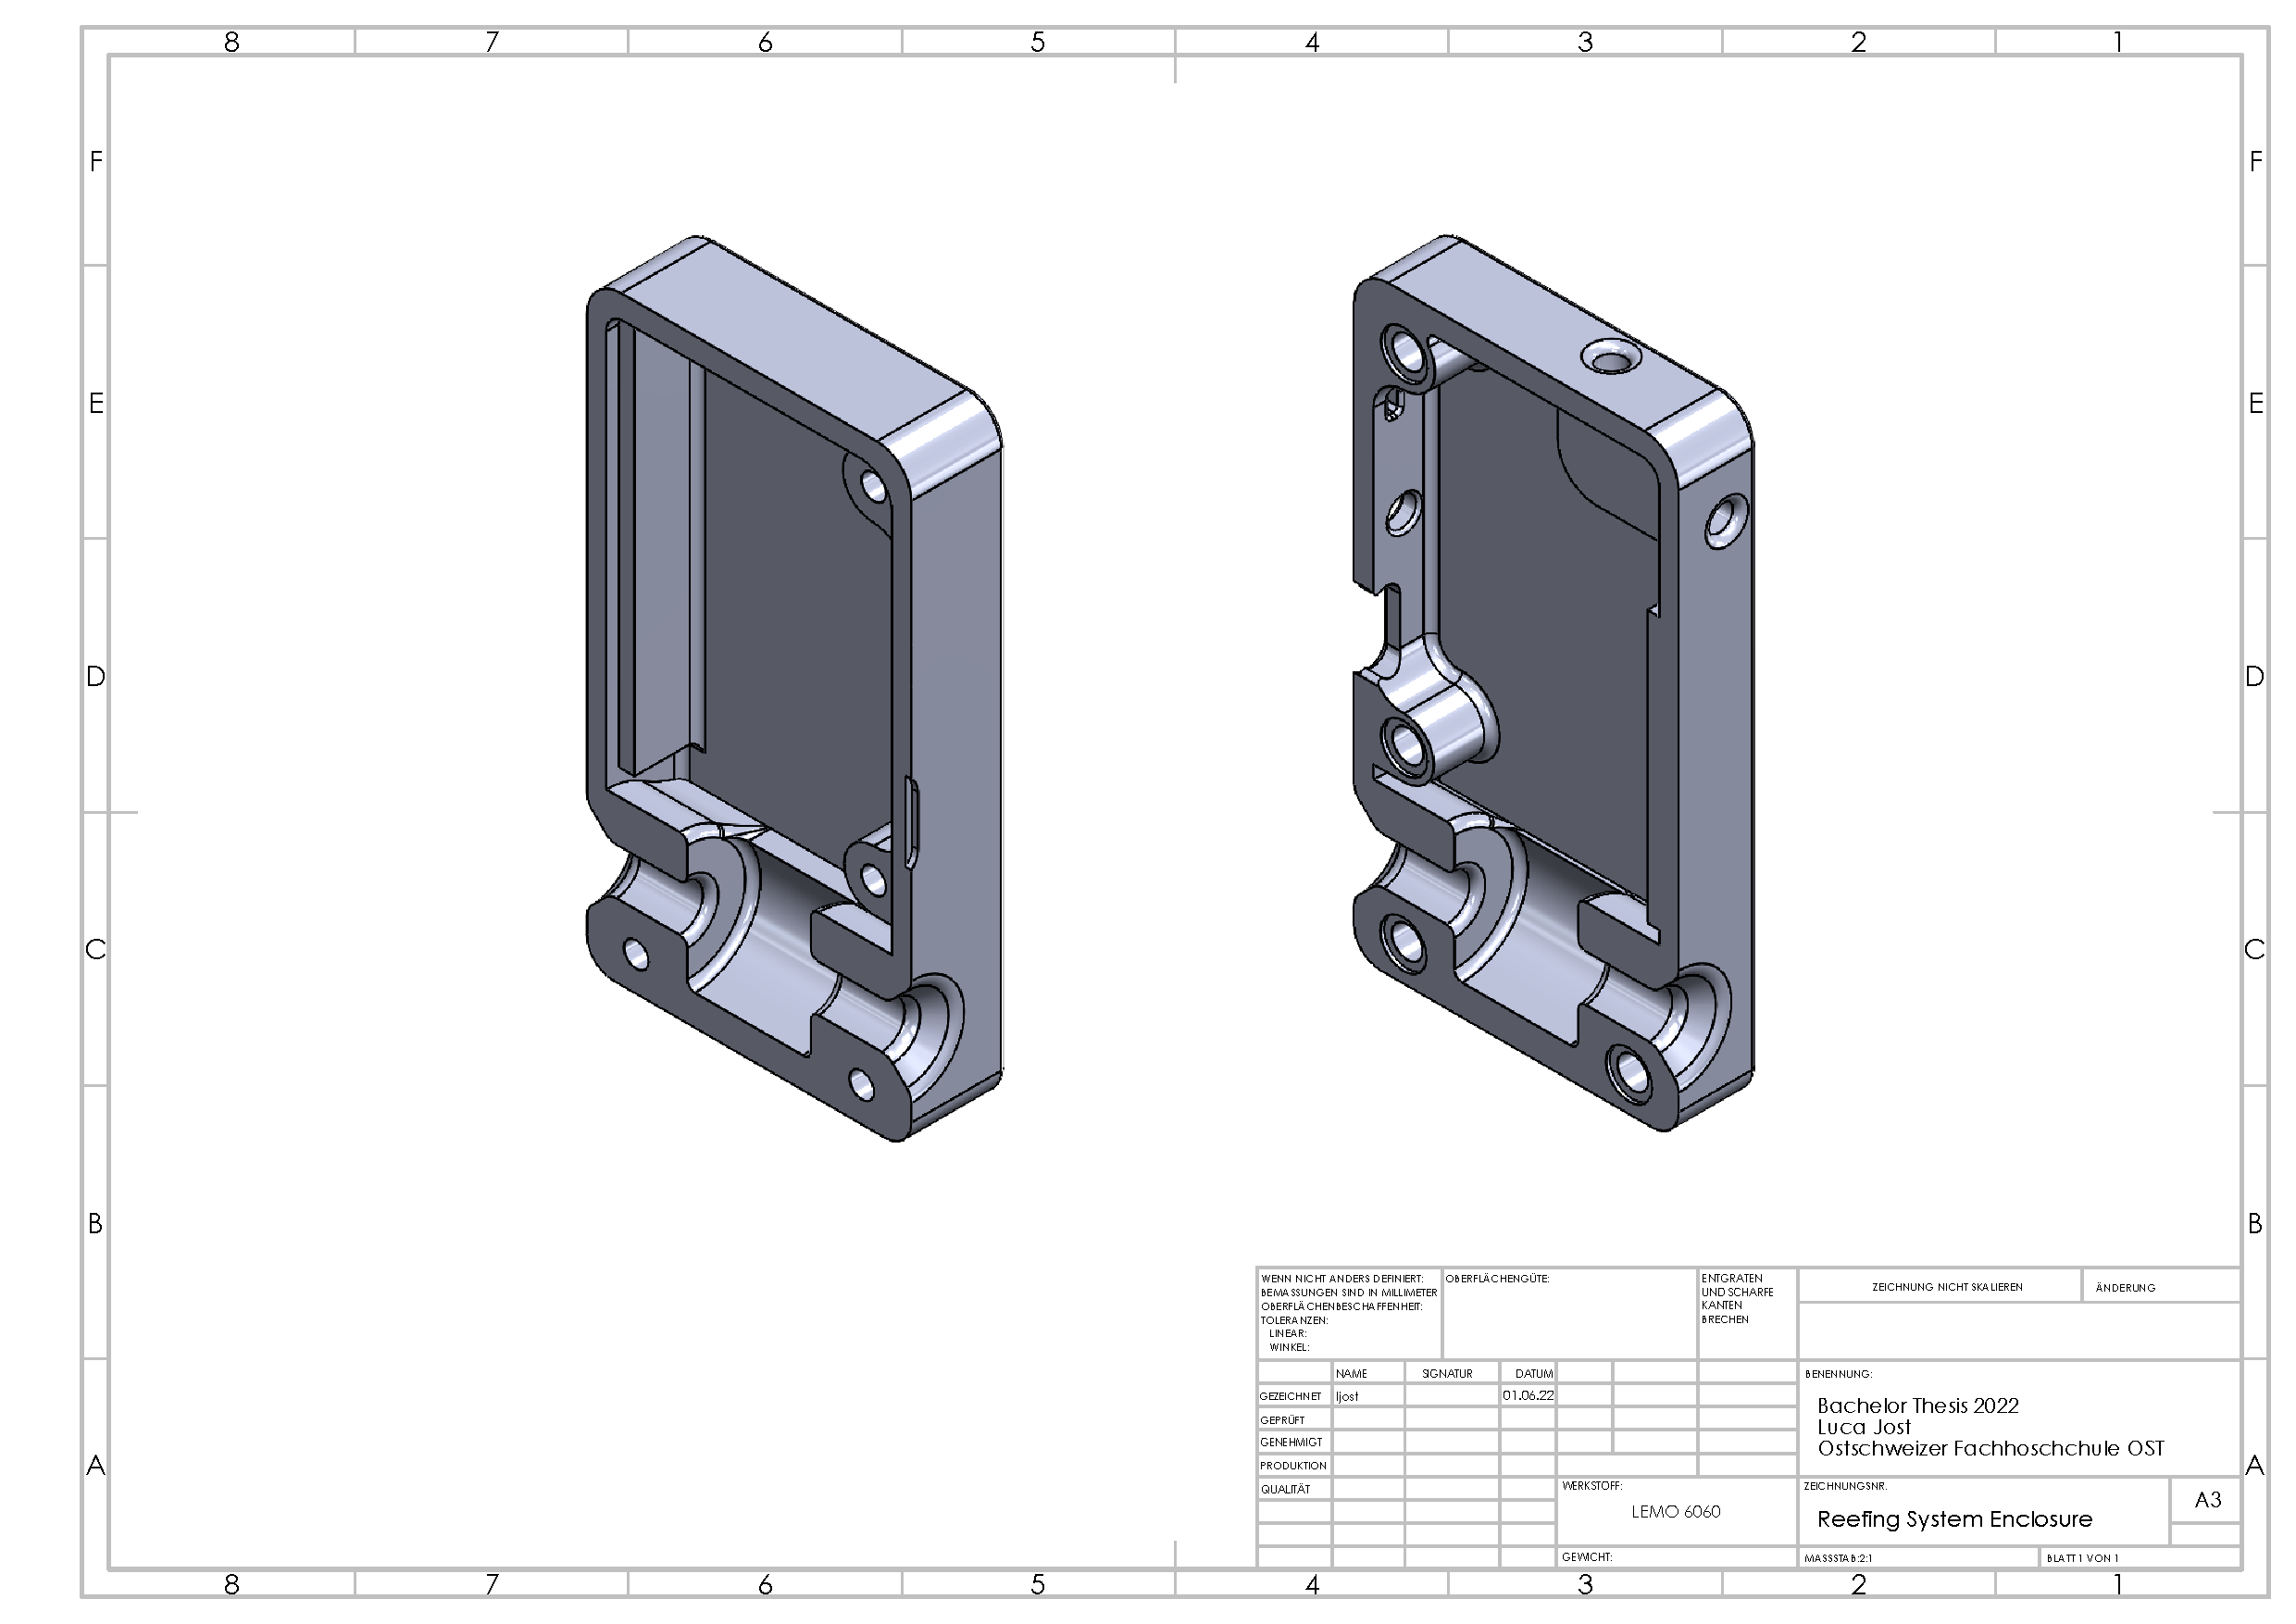
\includegraphics[angle=90, width=17.3cm, page=1]{appendix/Reefing System Mechanical}}
\end{adjustwidth}
\newpage

\section{Data Archive} \label{Data Archive}
All created files and documents of this project are publicly available on GitHub. An institution called \textbf{BA-OST-22} (\url{https://github.com/BA-OST-22}) has been created which contains repositories for each individual part of the project.
A quick description of the repositories including the associated web link is listed below:

\subsubsection{reefing-system-admin} \label{reefing-system-admin} \vspace{-0.2cm}
\begin{description}
  \item[Description:] This repository contains all confidential information of the project.\vspace{-0.25cm}
  \item[URL:] \url{https://github.com/BA-OST-22/reefing-system-admin}\vspace{-0.25cm}
  \item[Type:] Private\vspace{-0.25cm}
\end{description}

\subsubsection{reefing-system-docs} \vspace{-0.2cm}
\begin{description}
  \item[Description:] This repository contains all additional documentation of the project.\vspace{-0.25cm}
  \item[URL:] \url{https://github.com/BA-OST-22/reefing-system-docs}\vspace{-0.25cm}
  \item[Type:] Public\vspace{-0.25cm}
\end{description}

\subsubsection{reefing-system-hardware} \vspace{-0.2cm}
\begin{description}
  \item[Description:] This repository contains hardware and mechanical related documents.\vspace{-0.25cm}
  \item[URL:] \url{https://github.com/BA-OST-22/reefing-system-hardware}\vspace{-0.25cm}
  \item[Type:] Public\vspace{-0.25cm}
\end{description}

\subsubsection{reefing-system-firmware} \vspace{-0.2cm}
\begin{description}
  \item[Description:] This repository contains firmware source code written in C.\vspace{-0.25cm}
  \item[URL:] \url{https://github.com/BA-OST-22/reefing-system-firmware}\vspace{-0.25cm}
  \item[Type:] Public\vspace{-0.25cm}
\end{description}

\subsubsection{reefing-system-utilities} \vspace{-0.2cm}
\begin{description}
  \item[Description:] This repository contains all utilities for simulation, flight parsing and data plotting written in Python.\vspace{-0.25cm}
  \item[URL:] \url{https://github.com/BA-OST-22/reefing-system-utilities}\vspace{-0.25cm}
  \item[Type:] Public\vspace{-0.25cm}
\end{description}
